
\begin{wrapfigure}{r}{0.58\textwidth}
	\vspace*{-0.3cm}
	\includegraphics[page=10,width=0.97\linewidth]{Chapters/Ch4-BaseAnalysis/1_Exclusivity_Cuts/figures/eppi0.exclusive.pdf}
	\caption{MM$^2$ (epX) vs $\theta_X\pi$ 2D distribution.}
	\label{fig:MM2vsThetaXPi}
\end{wrapfigure}
After the selection of events with at least one electron, proton and two photons, it is time to take a look at the exclusive distributions.
The Fig.~\ref{fig:MM2vsThetaXPi} shows 2D distribution of MM$^2$ (epX) vs $\theta_{X\pi}$, where MM$^2$ (epX) is a missing mass squared of (epX) system and should have a peak near 0.0182 GeV$^2$, and $\theta_{X\pi}$ is an angle between expected and reconstructed pion.
The bright spot on the figure corresponds to the exclusive $ep\rightarrow~ep\pi^0$ events.
In order to reduce the background exclusivity cuts  need to be developed based on the conservation of energy and momentum.
The relevant 1D exclusive distributions are shown on the Fig.~\ref{fig:rawexclusive1} and \ref{fig:rawexclusive2}.

\begin{figure}[hbt]
	\centering
	\includegraphics[page=4,width=0.47\linewidth]{Chapters/Ch4-BaseAnalysis/1_Exclusivity_Cuts/figures/eppi0.exclusive.pdf}
	\includegraphics[page=5,width=0.47\linewidth]{Chapters/Ch4-BaseAnalysis/1_Exclusivity_Cuts/figures/eppi0.exclusive.pdf}

	\caption{Exclusive distributions for events with at least one electron, proton and two photons.}
	\label{fig:rawexclusive1}
\end{figure}

\begin{figure}[hbt]
	\centering
	\includegraphics[page=6,width=0.47\linewidth]{Chapters/Ch4-BaseAnalysis/1_Exclusivity_Cuts/figures/eppi0.exclusive.pdf}
	\includegraphics[page=8,width=0.47\linewidth]{Chapters/Ch4-BaseAnalysis/1_Exclusivity_Cuts/figures/eppi0.exclusive.pdf}
	
	\caption{Exclusive distributions for events with at least one electron, proton and two photons.}
	\label{fig:rawexclusive2}
\end{figure}

\subsection{Tight \texorpdfstring{$M_{\gamma\gamma} $} mass and transverse missing momenta cuts}

The first step is to use tighter $\gamma\gamma$ mass cut: $0.096<M_{\gamma\gamma}<0.168$ GeV, and take a look at the missing transverse momentum distributions (see Fig.~\ref{fig:ptdistributions}).
From momentum conservation law we expect transverse momentum to be zero, so we can apply cuts on $\Delta p_x$ and $\Delta p_y$ to further improve exclusive channel selection.
The cuts $|\Delta p_x|<0.2$ and $|\Delta p_y|<0.2$ correspond roughly to 4-5 $\sigma$.

\begin{figure}[hbt]
	\centering
	\includegraphics[page=24,width=0.47\linewidth]{Chapters/Ch4-BaseAnalysis/1_Exclusivity_Cuts/figures/eppi0.exclusive.pdf}
	\includegraphics[page=25,width=0.47\linewidth]{Chapters/Ch4-BaseAnalysis/1_Exclusivity_Cuts/figures/eppi0.exclusive.pdf}
	
	\caption{Exclusive distributions for events with at least one electron, proton and two photons.}
	\label{fig:ptdistributions}
\end{figure}

The exclusive distributions after tight $M_{\gamma\gamma}$ mass and transverse missing momenta cuts are shown on Fig.~\ref{fig:rawexclusive3} and display much stronger signal peaks on top of reduced background.

\begin{figure}[hbt]
	\centering
	\includegraphics[page=43,width=0.45\linewidth]{Chapters/Ch4-BaseAnalysis/1_Exclusivity_Cuts/figures/eppi0.exclusive.pdf}
	\includegraphics[page=44,width=0.45\linewidth]{Chapters/Ch4-BaseAnalysis/1_Exclusivity_Cuts/figures/eppi0.exclusive.pdf}
	
	\includegraphics[page=45,width=0.45\linewidth]{Chapters/Ch4-BaseAnalysis/1_Exclusivity_Cuts/figures/eppi0.exclusive.pdf}
    \includegraphics[page=47,width=0.45\linewidth]{Chapters/Ch4-BaseAnalysis/1_Exclusivity_Cuts/figures/eppi0.exclusive.pdf}

	\caption{Exclusive distributions after tight $M_{\gamma\gamma}$ mass and transverse missing momenta cuts .}
	\label{fig:rawexclusive3}
\end{figure}

\subsection{\texorpdfstring{$\theta_{X\pi}$} cut determination}

The cut on angle between expected and reconstructed pion is used in order to further reduce background.
To choose the value of the $\theta_{X\pi}$ cut the $MM^2(epX)$ distribution is analyzed at multiple $\theta_{X\pi}$ cut values and fit using gaussian+polynomial function as shown on Fig.~\ref{fig:mm2fordifferenttheta}.
From the fit we can estimate the number of good exclusive events (gaussian) and the number of background events (polynomial) and their dependence on $\theta_{X\pi}$ cut.
Fig.~\ref{fig:sigbgvsthetacutQ2} and~\ref{fig:sigbgvsthetacutxB} show the numbers of signal and background events as functions of $\theta_{X\pi}$ cut value for multiple bins in $Q^2$ and $x_B$.
These plots show that the cut $\theta_{X\pi}<2^\circ$ allows to select the most number of good events with the least background, and relaxing it beyond $2^\circ$ does not gain us any good exclusive events but increases background.


\begin{figure}[hbt]
	\centering
	\includegraphics[page=123,width=0.3\linewidth]{Chapters/Ch4-BaseAnalysis/1_Exclusivity_Cuts/figures/sigbg_eppi0.pdf}
	\includegraphics[page=125,width=0.3\linewidth]{Chapters/Ch4-BaseAnalysis/1_Exclusivity_Cuts/figures/sigbg_eppi0.pdf}
	\includegraphics[page=128,width=0.3\linewidth]{Chapters/Ch4-BaseAnalysis/1_Exclusivity_Cuts/figures/sigbg_eppi0.pdf}
	
	\includegraphics[page=130,width=0.3\linewidth]{Chapters/Ch4-BaseAnalysis/1_Exclusivity_Cuts/figures/sigbg_eppi0.pdf}
	\includegraphics[page=133,width=0.3\linewidth]{Chapters/Ch4-BaseAnalysis/1_Exclusivity_Cuts/figures/sigbg_eppi0.pdf}
	\includegraphics[page=135,width=0.3\linewidth]{Chapters/Ch4-BaseAnalysis/1_Exclusivity_Cuts/figures/sigbg_eppi0.pdf}
	
	\caption{$MM^2(epX)$ distributions for multiple $\theta_{X\pi}$ cut values.}
	\label{fig:mm2fordifferenttheta}
\end{figure}


\begin{figure}[hbt]
	\centering
	
	\includegraphics[width=0.32\linewidth,page=34]{Chapters/Ch4-BaseAnalysis/1_Exclusivity_Cuts/figures/sigbg_eppi0.pdf}
	\includegraphics[width=0.32\linewidth,page=51]{Chapters/Ch4-BaseAnalysis/1_Exclusivity_Cuts/figures/sigbg_eppi0.pdf}
	\includegraphics[width=0.32\linewidth,page=68]{Chapters/Ch4-BaseAnalysis/1_Exclusivity_Cuts/figures/sigbg_eppi0.pdf}
	
	\includegraphics[width=0.32\linewidth,page=85]{Chapters/Ch4-BaseAnalysis/1_Exclusivity_Cuts/figures/sigbg_eppi0.pdf}
	\includegraphics[width=0.32\linewidth,page=102]{Chapters/Ch4-BaseAnalysis/1_Exclusivity_Cuts/figures/sigbg_eppi0.pdf}
	\includegraphics[width=0.32\linewidth,page=119]{Chapters/Ch4-BaseAnalysis/1_Exclusivity_Cuts/figures/sigbg_eppi0.pdf}
	
	\caption{The numbers of signal (red markers) and background (black markers) events as functions of $\theta_{X\pi}$ cut value for multiple $Q^2$ bins.}
	\label{fig:sigbgvsthetacutQ2}
\end{figure}


\begin{figure}[hbt]
	\centering
	
	\includegraphics[width=0.32\linewidth,page=136]{Chapters/Ch4-BaseAnalysis/1_Exclusivity_Cuts/figures/sigbg_eppi0.pdf}
	\includegraphics[width=0.32\linewidth,page=153]{Chapters/Ch4-BaseAnalysis/1_Exclusivity_Cuts/figures/sigbg_eppi0.pdf}
	\includegraphics[width=0.32\linewidth,page=170]{Chapters/Ch4-BaseAnalysis/1_Exclusivity_Cuts/figures/sigbg_eppi0.pdf}
	
	\includegraphics[width=0.32\linewidth,page=187]{Chapters/Ch4-BaseAnalysis/1_Exclusivity_Cuts/figures/sigbg_eppi0.pdf}
	\includegraphics[width=0.32\linewidth,page=204]{Chapters/Ch4-BaseAnalysis/1_Exclusivity_Cuts/figures/sigbg_eppi0.pdf}
	
	\caption{The numbers of signal (red markers) and background (black markers) events as functions of $\theta_{X\pi}$ cut value for multiple $x_B$ bins.}
	\label{fig:sigbgvsthetacutxB}
\end{figure}

\clearpage

\subsection{Final exclusivity cuts}

The list of final exclusive cuts is following:
\begin{itemize}
	\item $\Delta p_x<0.2$ GeV
	\item $\Delta p_y<0.2$ GeV
	\item $\theta_{X\pi}<2^\circ$
	\item $0.096<M_{\gamma\gamma}<0.168$ GeV
	\item $MM^2(epX)<0.5$ GeV$^2$
\end{itemize}

Exclusive distributions after all exclusivity cut except $MM^2(epX)<0.5$ GeV are shown on Fig.~\ref{fig:finalexclusive}

\begin{figure}[hbt]
	\centering
	
	\includegraphics[page=82,width=0.32\linewidth]{Chapters/Ch4-BaseAnalysis/1_Exclusivity_Cuts/figures/eppi0.exclusive.pdf}
	\includegraphics[page=83,width=0.32\linewidth]{Chapters/Ch4-BaseAnalysis/1_Exclusivity_Cuts/figures/eppi0.exclusive.pdf}
	\includegraphics[page=84,width=0.32\linewidth]{Chapters/Ch4-BaseAnalysis/1_Exclusivity_Cuts/figures/eppi0.exclusive.pdf}
	\caption{Exclusive distributions after all exclusivity cuts .}
	\label{fig:finalexclusive}
\end{figure}

